
\documentclass[a4paper, 12pt, oneside]{uet_thesis}  
\graphicspath{{Figures/}}  
\usepackage{listings}
\usepackage{color}

\definecolor{dkgreen}{rgb}{0,0.6,0}
\definecolor{gray}{rgb}{0.5,0.5,0.5}
\definecolor{mauve}{rgb}{0.58,0,0.82}

\lstset{frame=none,
  language=SQL,
  aboveskip=3mm,
  belowskip=3mm,
  showstringspaces=false,
  columns=flexible,
  basicstyle={\small\ttfamily},
  numbers=none,
  numberstyle=\tiny\color{gray},
  keywordstyle=\color{blue},
  commentstyle=\color{dkgreen},
  stringstyle=\color{mauve},
  breaklines=true,
  breakatwhitespace=true,
  tabsize=3
}
\usepackage[square, numbers, comma, sort&compress]{natbib}  
\usepackage{xcolor}

\usepackage[document]{ragged2e}

\usepackage{verbatim} 


\usepackage{url}
\usepackage{natbib}


\hypersetup{urlcolor=blue, colorlinks=true}  

\usepackage[compact]{titlesec}
\titlespacing{\section}{0pt}{*0}{*0}
\titlespacing{\subsection}{0pt}{*0}{*0}
\titlespacing{\subsubsection}{0pt}{*0}{*0}

\setlength{\parskip}{6pt}

%% ----------------------------------------------------------------
\usepackage{titlesec}

\titleformat{\chapter}[block]
  {\normalfont\huge\bfseries}{\thechapter.}{0.5em}{\Huge}
\titlespacing*{\chapter}{0pt}{-19pt}{0pt}
\begin{document}
\setcounter{chapter}{0}
\frontmatter	  % Begin Roman style (i, ii, iii, iv...) page numbering

% Set up the Title Page
\title  {Final Year Project Management System}
\session {2021-- 2025}
\advisor {Mr. Nauman Babar}
\authors {  Abdul Mateen \\ \quad 2021-CS-190 }

\addresses  {\deptname \\ \univname}  % Do not change this here, instead these must be set in the "Thesis.cls" file, please look through it instead
\date       {\today}
\subject    {}
\keywords   {}

\maketitle
%% ----------------------------------------------------------------

\setstretch{1.3}  % It is better to have smaller font and larger line spacing than the other way round

% Define the page headers using the FancyHdr package and set up for one-sided printing
\fancyhead{}  % Clears all page headers and footers
\rhead{\thepage}  % Sets the right side header to show the page number
\lhead{}  % Clears the left side page header

\pagestyle{fancy}  % Finally, use the "fancy" page style to implement the FancyHdr headers



%% ----------------------------------------------------------------
\pagestyle{fancy}  %The page style headers have been "empty" all this time, now use the "fancy" headers as defined before to bring them back

%% ----------------------------------------------------------------
\lhead{\emph{Contents}}  % Set the left side page header to "Contents"
\begingroup % start a TeX group
\color{black}% or whatever color you wish to use
\tableofcontents
\endgroup
% \tableofcontents  % Write out the Table of Contents

%% ----------------------------------------------------------------
\lhead{\emph{List of Figures}}  
\listoffigures  



%% ----------------------------------------------------------------
\pagestyle{fancy} 
\onehalfspacing
\lhead{\emph{Acknowledgements}}  
\acknowledgements{
{
I am grateful to Allah Almighty that He provided me with the strength and power to
complete this project in time.
I am thankful to Mr. Samyan Wahla for the supervision, guidance, and care he provided
throughout the project for making out the best project I could, by enlightening myself with
the techniques to manage my work by making a schedule beforehand.
Base Theory and presenting concepts in a manner that helped me complete this project
with great ease.
}}
\pagebreak
%---------------------------------------------------------------

\addtotoc{Abstract}  % Add the "Abstract" page entry to the Contents
\lhead{\emph{Abstract}}  
\abstract{
The main purpose of this project was to understand the working of a database management system and the configuration of the database with a front-end by making a desktop-based Management System. A database schema was used provided by the supervisor, Mr. Samyan Wahla. For data population, the data were entered manually by the front end of the project.
\\
For background research purposes a report was provided by Mr. Samyan Wahla (Lecturer in Computer Science department UET Lahore). In which whole working procedure, of the committee for management of the final year project of the Department of Computer Science UET Lahore, is streamlined. 
\\
This system is an automation of the working procedure followed by the committee for management of the final year project of the Department of Computer Science UET Lahore. This system supports the management of students, advisors, projects, groups, and evaluations. And all of tese tasks are now automated and the only thing users need to do is enter data in the system and the rest will be managed by a database configured in our system.
}

\pagebreak
%---------------------------------------------------------------
\mainmatter	 
\chapter{Introduction}
\lhead{\emph{Introduction}}  
\section{Description}
The manangement of Final year project is done in every University. Where the Data of Student Evaluations are managed by hand on registers. Inserting ,Deleting and Managing data is so inefficient. Due to which there is a large chance of errors in that case there is need of a such a system which can automate the process. Computer Science Department of UET Lahore has a mannual system and there is need to make a software application so that this process is done by desktop based application integrated with Database. In final year project management system the Application needs to maintain the students, groups and project, evaluations of those groups. The evaluations of each group is done by advisors. Student make a group of at least two students and a Advisor Board is Assigned to them which supervise there project. The board consists of Main Advisor , Co advisor  and industry advisors.\\
The Main Advisor is the one who maintains manages , supervise, evaluates and leads the group. Where Co advisor and industry advisor Guides the group to make a life solving project. There are multiple evaluations of each group and this record help us in Final Evaluation. \\
Records are maintained according to the date a student is assigned to a group or the project is assigned to a group. Multiple group may work on same project similarly Same advisor can be assigned to multiple groups. The faculty added to the Advisor Data are according to there designation forexample Assistant professor, Lecturer etc.  


\section{Motivation}
The motivation of the project is to learn how Databases work and how to maintain Data in tables to easily use them in the future. The project is implement on C# .NET Framework  and SQL Server was used as Database. MoreOver, PDF report is generated at the last using ItextSharp which contains useful information related to groups and projects.  


\section{Target Audience}
The target audience of this project is all the Universities where final year projects 
managed on paper. This desktop application will help them add students ,Advisors, Create groups and manage their evalations on anytime. An advisor can supervise multiple projects and evaluate them. Students are evaluted on group based and hence assigned equal marks.
\clearpage
%-----------------------------------------------------------------
\chapter{Operational Details}
\lhead{\emph{Operation Details}}  
The management system is made for the single user which is most probably admin . Following are the details that the admin can :
The Application is made for a single User who is Admin and manages all the System. Following are listed all the functionalities a user can perform.

\begin{enumerate}
    \item The Admin can Add and Update all details of each Student. 
    \item Also just like Students user can add Advisors.
    \item All listed projects will be added by admin and he will be able to update there title or discription.
    \item Group will be created by admin and Assigned one of the projects.
    \item Admin can Delete or remove a member from the group.
    \item Evalutions of Each group will be taken by Admin and marks are added for each evalution.
    \item Pdf Reports are Generated by Admin to have a look at the results of each group.
\end{enumerate}
\clearpage
%-------------------------------------------

\chapter{Database Design}
\lhead{\emph{DataBase Design}}  
\begin{figure}[h]
    \centering
    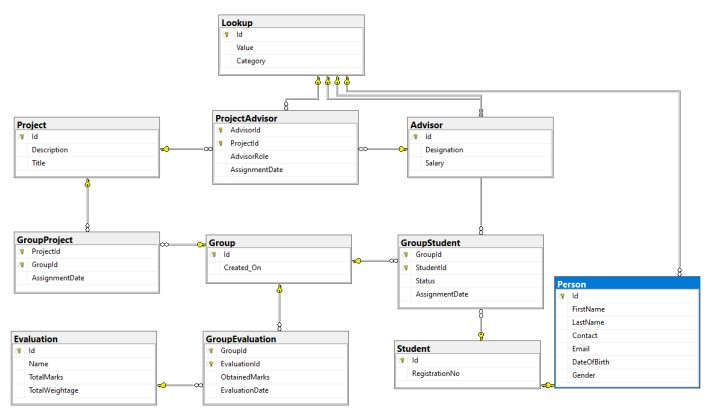
\includegraphics[width=1\textwidth]{Figures/DB_.jpg}
    \caption{Database Design of System}
    \label{fig:my_label}
\end{figure}

\section{Lookup}
Lookup Table provided details about different table like gender of advisor, Student and Designation of Advisors and status of students in each group.

\section{Person}
Person consist of details that a student or advisor need. The person Id act as Key to Student and Advisor Table. The data of student is stored in the person table if student is deleted than its related information in person table is also deleted.

\section{Student}
Student table consist of student registration number and id through which it is linked to person table.

\section{Group}
Group contains information of its id and the date it is created on. 

\section{GroupStudent}
Group student table has the information of the student which group it has joined and if he is still active in that group.

\section{Project}
This table has project id as primary key ,title  and its description.

\section{GroupProject}
The Group Project consist of project id and id of group it i

\section{Evalaution}
Evaluations consists of id and total marks and its weightage.

\section{GroupEvaluation}
GroupEvaluations consists of obtained marks of each evaluation of a group.

\section{Advisor}
The advisor relation consists of the advisor's designation and the salray. Id acts as the primary key of the relation. The designation is a foriegn key for the parent Lookup table.

\section{ProjectAdvisor}
Project Advisor table consists of advisor of that is assigned to each group. Along with there roles. The project and Advisor id act as primary key.

\clearpage


%-----------------------------------------------------------------
\chapter{Graphic User Interface}
\lhead{\emph{Graphic User Interface}}  

\section{Add Students}
\begin{figure}[h]
    \centering
    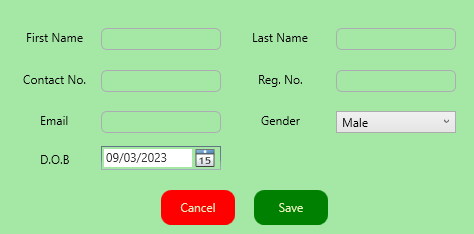
\includegraphics[width=1\textwidth]{Figures/AddStudent.png}
    \caption{Add Student Window}
    \label{fig:my_label}
\end{figure}

\section{Update Student}
\begin{figure}[h]
    \centering
    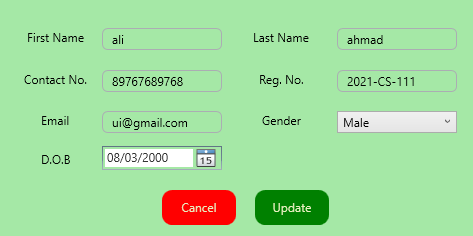
\includegraphics[width=1\textwidth]{Figures/UpdateStudent.png}
    \caption{Update Student Window}
    \label{fig:my_label}
\end{figure}

\clearpage

\section{View Students}
\begin{figure}[h]
    \centering
    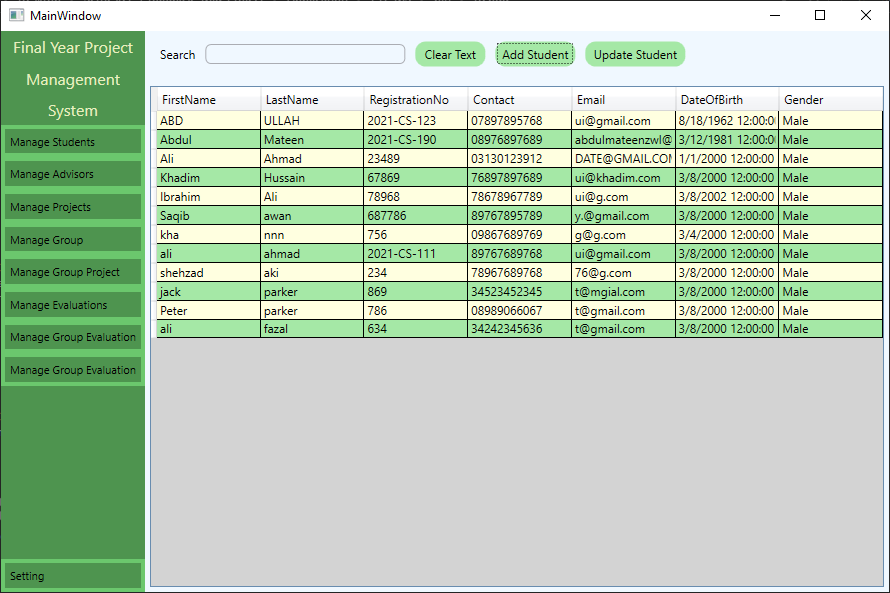
\includegraphics[width=1\textwidth]{Figures/ViewStudents.png}
    \caption{View Student Window}
    \label{fig:my_label}
\end{figure}


\section{Add Advisor}
\begin{figure}[h]
    \centering
    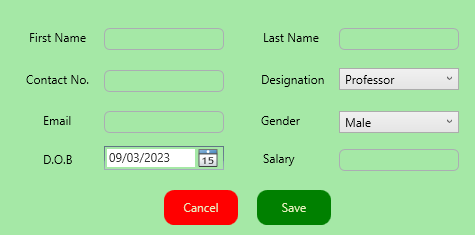
\includegraphics[width=1\textwidth]{Figures/AddAdvisor.png}
    \caption{Add Advisor Window}
    \label{fig:my_label}
\end{figure}
\clearpage

\section{Update Advisor}
\begin{figure}[h]
    \centering
    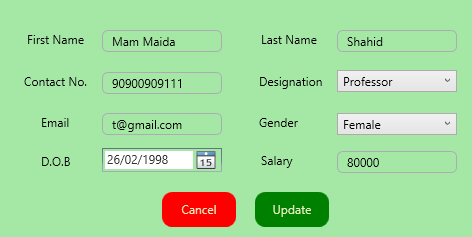
\includegraphics[width=1\textwidth]{Figures/UpdateAdvisor.png}
    \caption{Update Advisor Window}
    \label{fig:my_label}
\end{figure}


\section{View Advisors}
\begin{figure}[h]
    \centering
    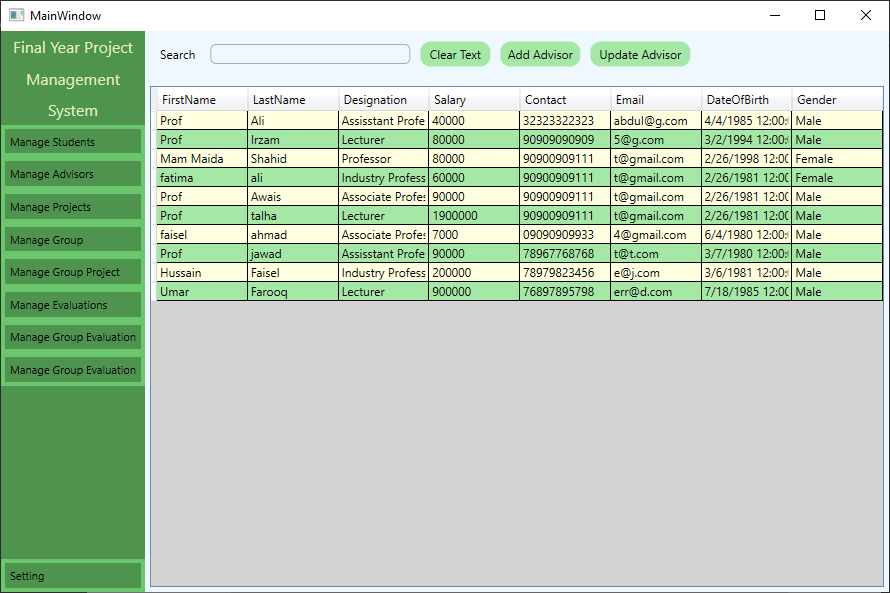
\includegraphics[width=1\textwidth]{Figures/ViewAdvisors.png}
    \caption{View All Advisors Window}
    \label{fig:my_label}
\end{figure}
\clearpage

\section{Add Project}
\begin{figure}[h]
    \centering
    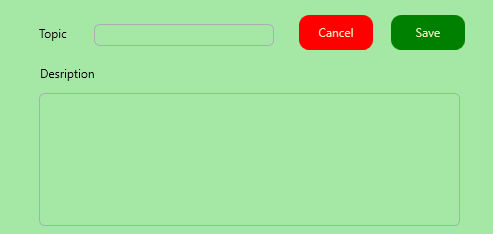
\includegraphics[width=1\textwidth]{Figures/AddProject.png}
    \caption{Add Project Window}
    \label{fig:my_label}
\end{figure}

\section{View All Project}
\begin{figure}[h]
    \centering
    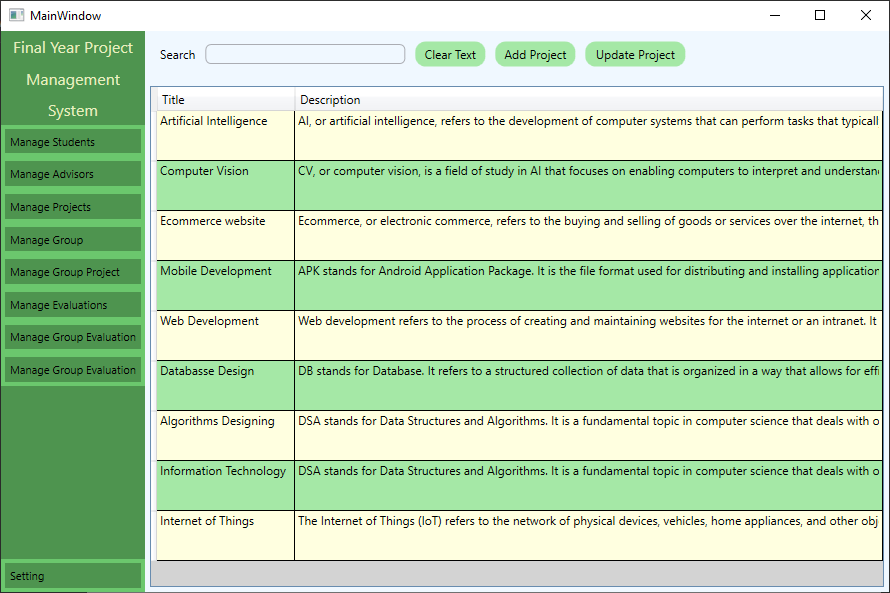
\includegraphics[width=1\textwidth]{Figures/ViewProject.png}
    \caption{View Project Window}
    \label{fig:my_label}
\end{figure}
\clearpage

\section{Update Project}
\begin{figure}[h]
    \centering
    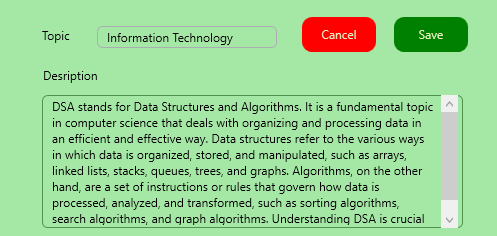
\includegraphics[width=1\textwidth]{Figures/UpdateProject.png}
    \caption{Update Project Window}
    \label{fig:my_label}
\end{figure}

\section{View Groups}
\begin{figure}[h]
    \centering
    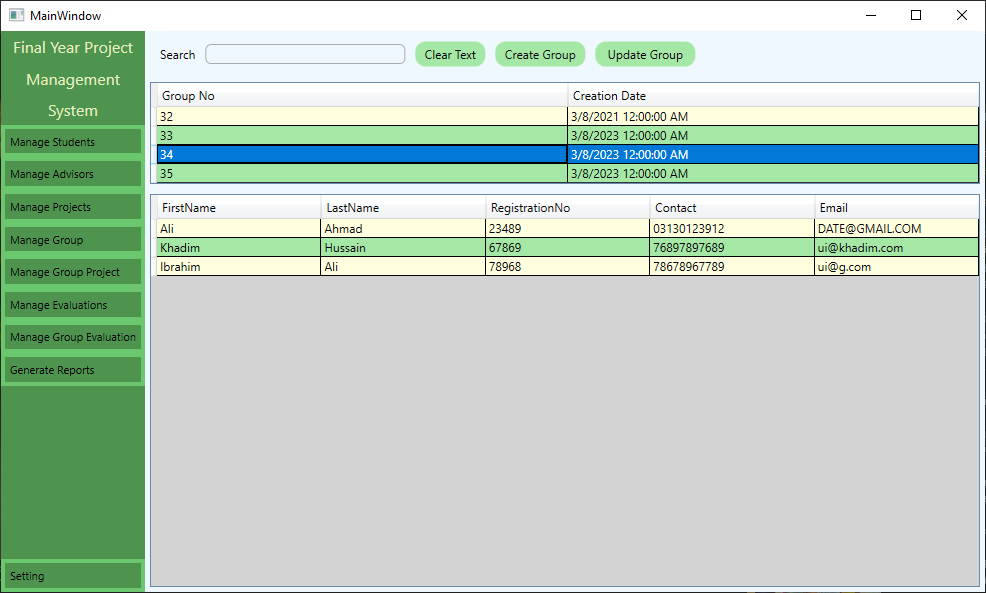
\includegraphics[width=1\textwidth]{Figures/viewGroups.png}
    \caption{View Group Window}
    \label{fig:my_label}
\end{figure}
\clearpage

\section{Add Group}
\begin{figure}[h]
    \centering
    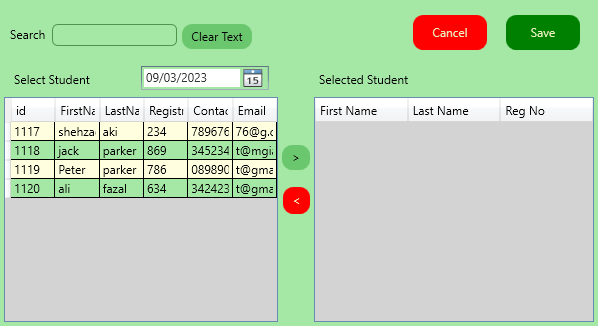
\includegraphics[width=1\textwidth]{Figures/AddGroup.png}
    \caption{Add Group Window}
    \label{fig:my_label}
\end{figure}

\section{Assign Project}
\begin{figure}[h]
    \centering
    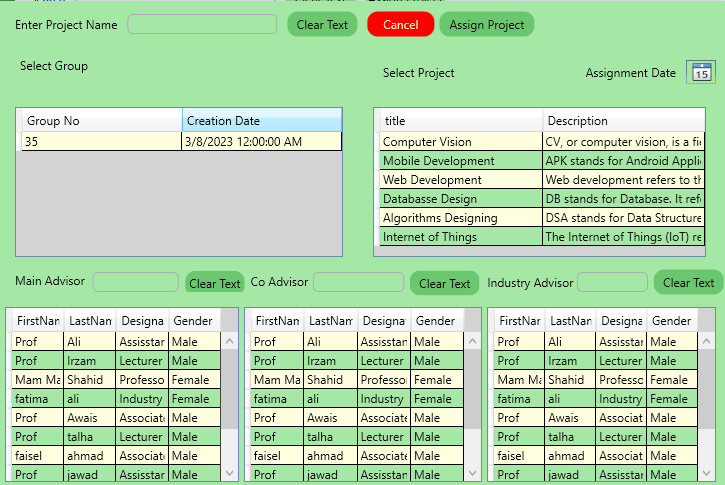
\includegraphics[width=1\textwidth]{Figures/AddAssignProject.png}
    \caption{Assign Project Window}
    \label{fig:my_label}
\end{figure}
\clearpage


\section{View Evaluations}
\begin{figure}[h]
    \centering
    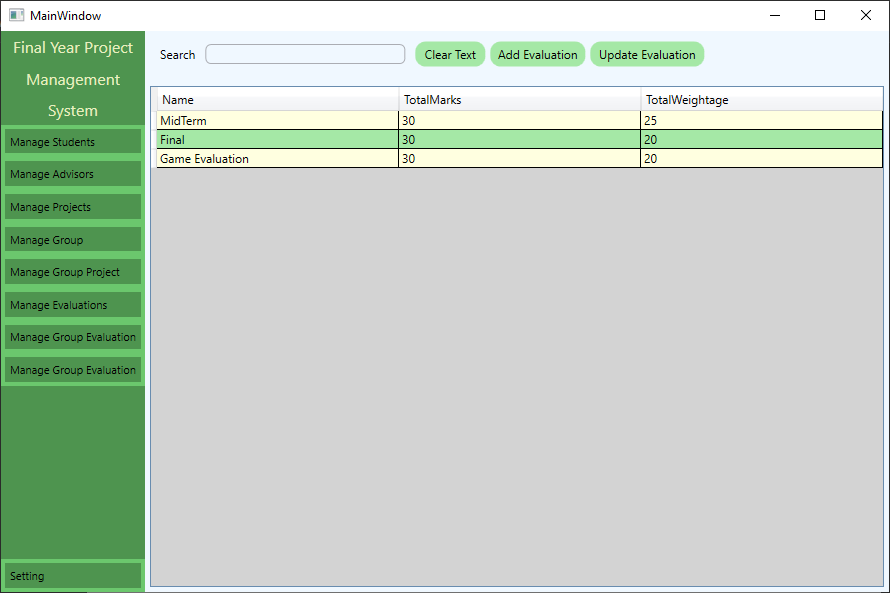
\includegraphics[width=1\textwidth]{Figures/ViewEvaluations.png}
    \caption{View Evaluations Window}
    \label{fig:my_label}
\end{figure}

\section{Add Evaluations}
\begin{figure}[h]
    \centering
    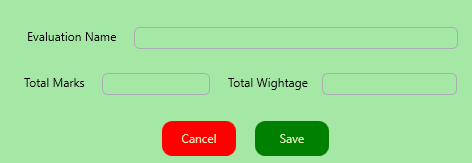
\includegraphics[width=1\textwidth]{Figures/AddEvaluation.png}
    \caption{Add Evaluations Window}
    \label{fig:my_label}
\end{figure}
\clearpage



\section{Update Evaluations}
\begin{figure}[h]
    \centering
    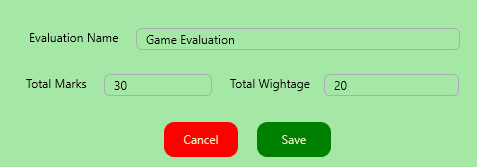
\includegraphics[width=1\textwidth]{Figures/UpdateEvaluation.png}
    \caption{Update Evaluations Window}
    \label{fig:my_label}
\end{figure}

\section{View Group Evaluations}
\begin{figure}[h]
    \centering
    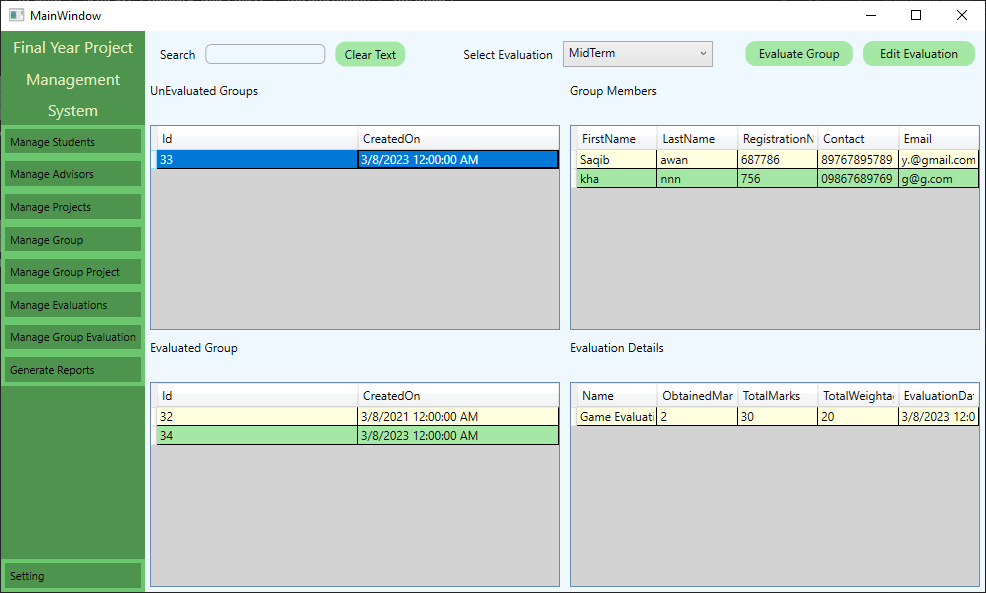
\includegraphics[width=1\textwidth]{Figures/ViewGroupEvaluation.png}
    \caption{View Group Evaluations}
    \label{fig:my_label}
\end{figure}
\clearpage



\section{Add Group Evaluations}
\begin{figure}[h]
    \centering
    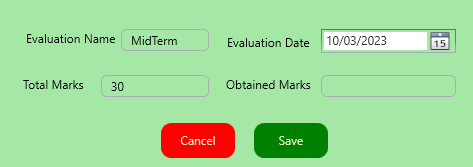
\includegraphics[width=1\textwidth]{Figures/AddEvaluateGroup.png}
    \caption{Add Evaluations Window}
    \label{fig:my_label}
\end{figure}

\section{Update Group Evaluation}
\begin{figure}[h]
    \centering
    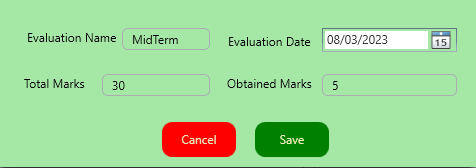
\includegraphics[width=1\textwidth]{Figures/UpdateGroupEvaluation.png}
    \caption{Update Group Evaluations Window}
    \label{fig:my_label}
\end{figure}
\clearpage

\section{Generate Report}
\begin{figure}[h]
    \centering
    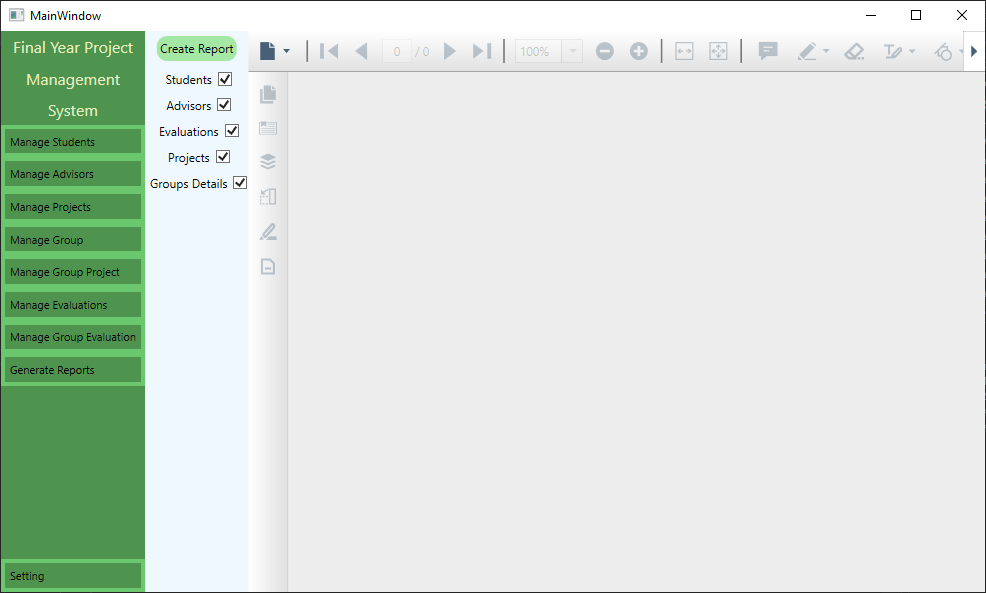
\includegraphics[width=1\textwidth]{Figures/Generate Report.png}
    \caption{Generate Report Window}
    \label{fig:my_label}
\end{figure}
\clearpage

%-----------------------------------------------------------------
\chapter{Testing}
\lhead{\emph{Testing}}  
The Application is tested at each and every stage multiple times. The queries used for are tested on ms SQL Server first. The Graphic User interface is responsive to a large to extinct. All the validations are checked under multiple conditions and values. The major challenge is to first time work with DataBase. And test the results of each query. There are some problems in deleting record of any tuple if is being used by any other table. The Application is totally responsive by using Grids in WPF.

\clearpage

\chapter{Limitations}
\lhead{\emph{Limitations}}  
The following are the limitations of the project:
\begin{enumerate}
    \item The application is made for Single User who is admin and manages all the records.
    \item The Data Entered by the admin is unable to delete in any way.
    \item Group can not be edited ie. Students in each group can not be edited.
    \item Once a group is assigned advisor can not be edited.
    \item There is no verification system that if the number or email provided by the student or advisor is valid.
\end{enumerate}
\clearpage

\chapter{Conclusion}
\lhead{\emph{Conclusion}}  
The Final Year Projects Management system Made for DataBase Mangement system Lab for learning purpose provided great experience to learn and understand basics of DataBase and learn how database is used in real life. The Project help me understand storing and retrieving large amounts of data to change it using Graphic User Interface.


\end{document} 